\documentclass{article}

\usepackage[nottoc]{tocbibind}
\usepackage[a4paper, total={7.7in, 10in}]{geometry}
\usepackage[utf8]{inputenc}
\usepackage{amsmath,amssymb}
\usepackage{chngpage}
\usepackage{graphicx}
\DeclareMathOperator{\E}{\mathbb{E}}
\DeclareMathOperator{\D}{\mathbb{D}}

\begin{document}

\title{
    Term Project 2018: Collision avoidance using deep reinforcment learning. 
}
\maketitle


\section{Introduction}

Indoor navigation and collision avoidance is under significant 
development in the recent literature. Among several applications,
these tasks are designed to help mobile robots, quadrotors and other
similar devices to operate in open-world environments. The majority
of approaches uses SLAM, depth sensors and stereo/monocular cameras.
Using sophisticated sensors imposes additional costs, as well as 
increases weight of the devices. On the other side, using monocular
cameras is difficult, since we need to estimate additional information,
like depth and environment structure.

In this study we base on the paper \cite{cad2rl},
and explore application of reinforcement learning for 
indoor navigation, without explicit 3D-modeling of unknown environment
during application. However, during training several environments are 
used, though model does not know about them. To do that, we use
Unreal Engine and quadrotor simulator AirSim.
Essentially, the project is about collision avoidance in AirSim +
UnrealEngine environment, using deep reinforcement learning.


\subsection{Unreal Engine and AirSim}

The Unreal Engine is a game engine developed by Epic Games.
It is written in C++ and proved itself as cross-platform, reasonably
open and highly comfortable in use.

AirSim  is  an  open-source  platform \cite{airsim2017fsr} by Microsoft,
that allows to model quadorotors or vehicles in different environments, 
on top of Unreal Engine.
It is inspired by several previous simulators (see
related work), and proved to be very useful in this project development.

\subsection{Structure description}

The rest of the study is organized in the following way. 

{\bf TODO: write as it is organized.}


\section{Introduction to reinforcement Learning}

\subsection{General description. }

\subsection{Markov Decision Process}

TBD

\subsection{Policy Iteration. Value Iteration.}

TBD

\subsection{Monte-carlo, Temporal Difference, $TD(\lambda)$}

TBD

\subsection{Model-free control. On-policy and Off-policy.}

TBD

\subsubsection{SARSA}

TBD

\subsubsection{Q-learning}

TBD

\subsection{Value function approximation. Deep Q-learning}


\subsubsection{Tricks to make it work}

TBD

\subsection{Policy Gradient Methods. Actor-Critic.}

TBD

\subsubsection{REINFORCE}

TBD

\subsubsection{Actor Critic}

TBD

\subsubsection{Advantage Actor Critic}

TBD

\subsubsection{TD Actor Critic}

TBD

\subsubsection{$TD(\lambda)$ Actor Critic}

TBD

\subsubsection{Natural Actor Critic}

TBD

\subsection{Exploration and Exploitation}

TBD

\subsubsection{Multi-Armed Bandits}

\subsubsection{Contextual Bandits}

\subsubsection{MDPs}

\subsection{Integrated Learning and Planning}

\subsection{Partially Observed MDPs}

\subsection{Inverse Reinforcement Learning}

\subsection{Multi-agent reinforcement learning}

\subsection{Trusted Region Policy Optimization (TRPO)}

\subsection{Asynchronous Approaches: A3C, D4PG}


\section{Description of the framework architecture}

Architecture consists of the following classes. The main character is
Agent, which can act, observe and train.
To make agent more readable, we separated History and
ExperienceReplayMemory into separated classes.
With the goal of making substitutable actions and rewards,
we introduced classes ActionSpace and Reward.
To control exploration-exploatation dilemma, we created module to
handle exploration (with Explorer classes).

Our implementation uses deep learning libraries CNTK
and TensorFlow (with Tensorboard).

\section{Considered Environments}

The following environments were considered under Linux:
\begin{enumerate}
    \item Blocks.
    \item Cave.
    \item Landscape Mountains.
    \item Corridor.
\end{enumerate}

 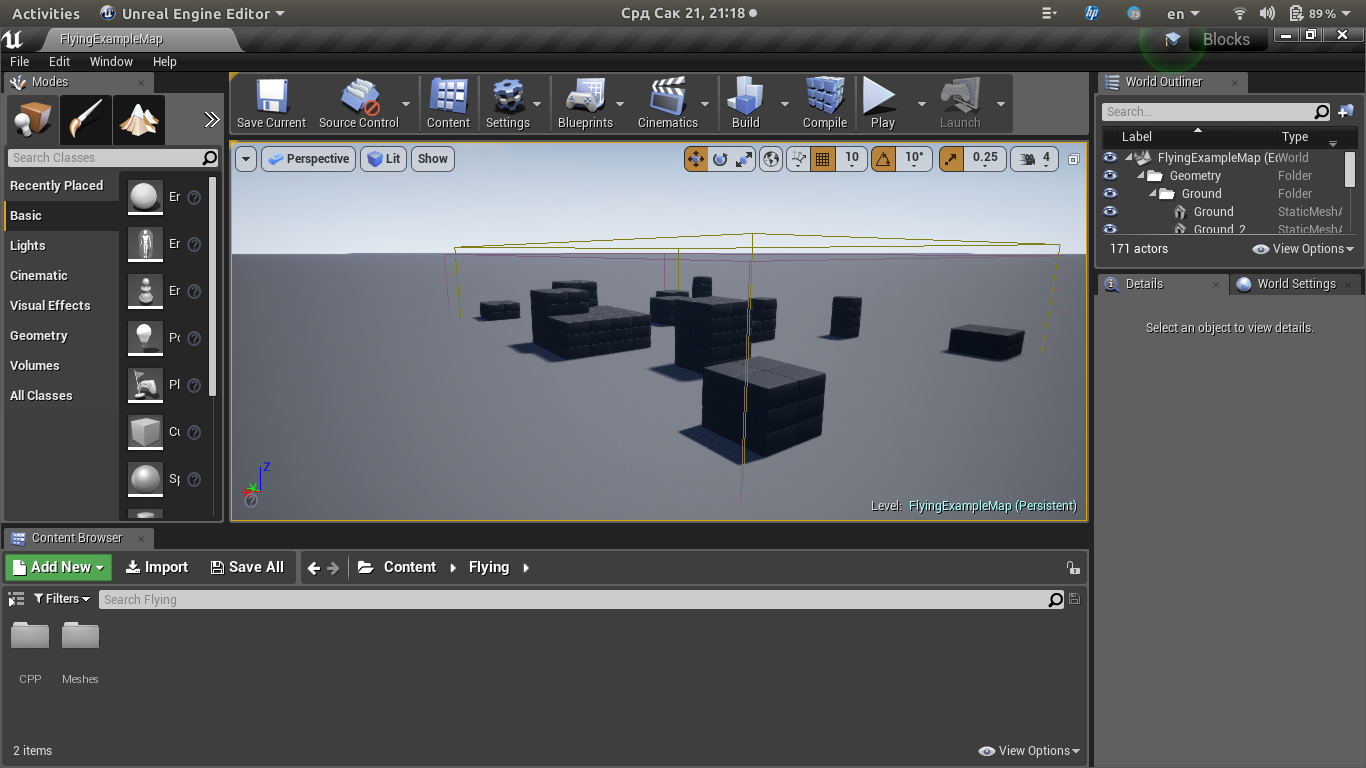
\includegraphics[scale=0.1]{environments/blocks.png}
 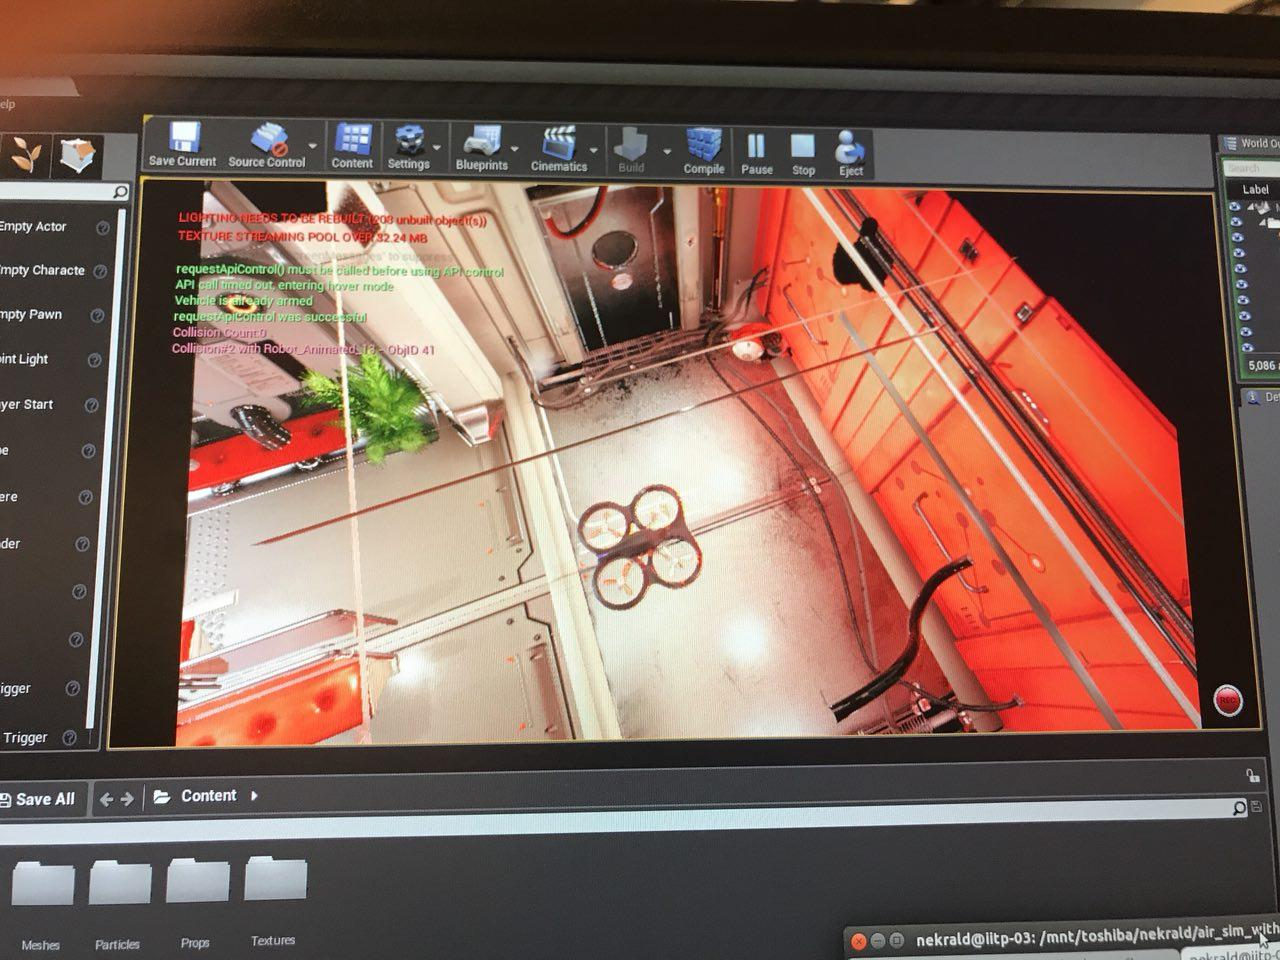
\includegraphics[scale=0.1]{environments/corridor.jpg}
 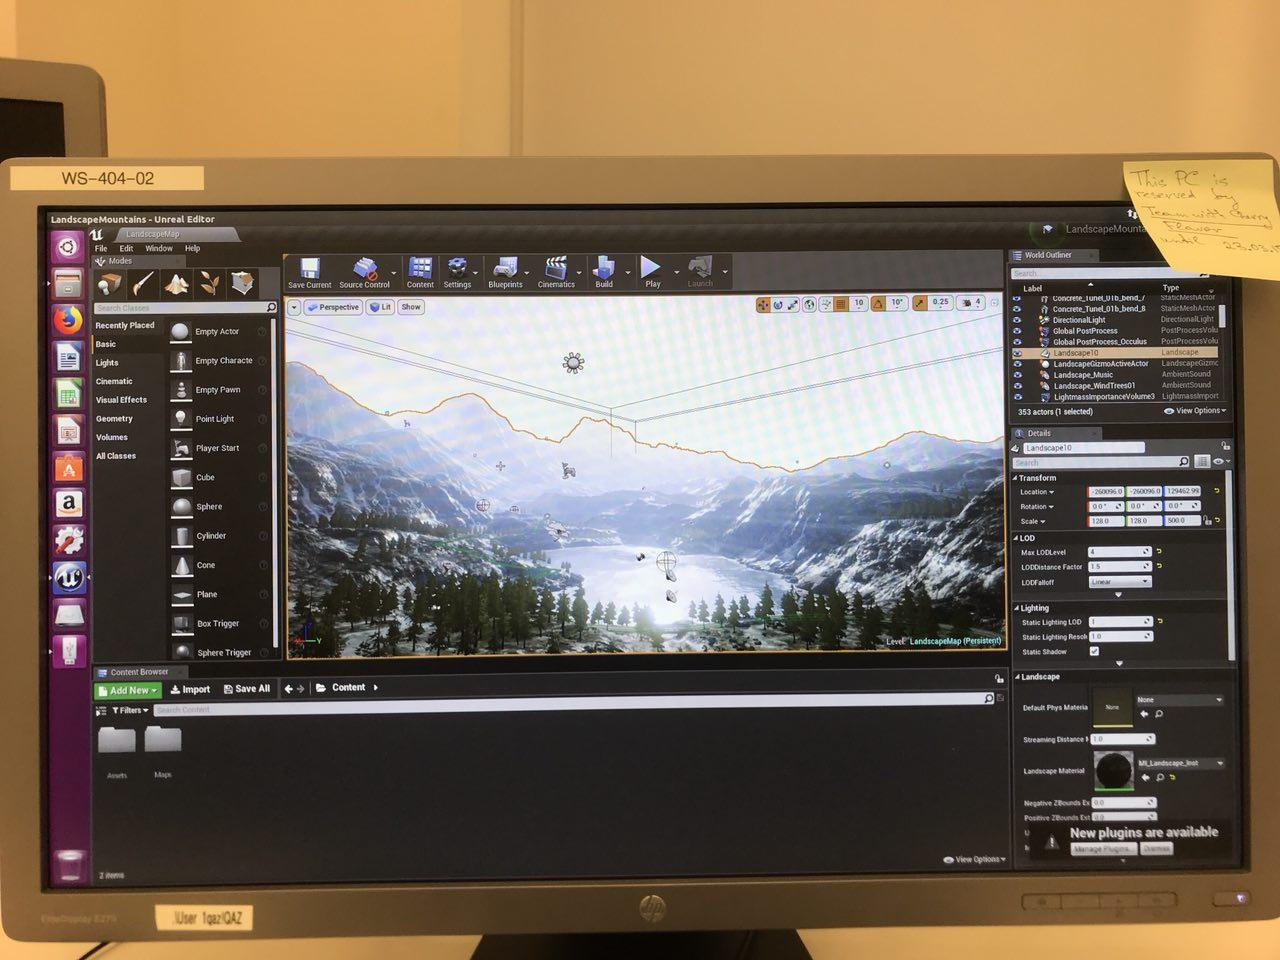
\includegraphics[scale=0.1]{environments/landscape.jpg}
 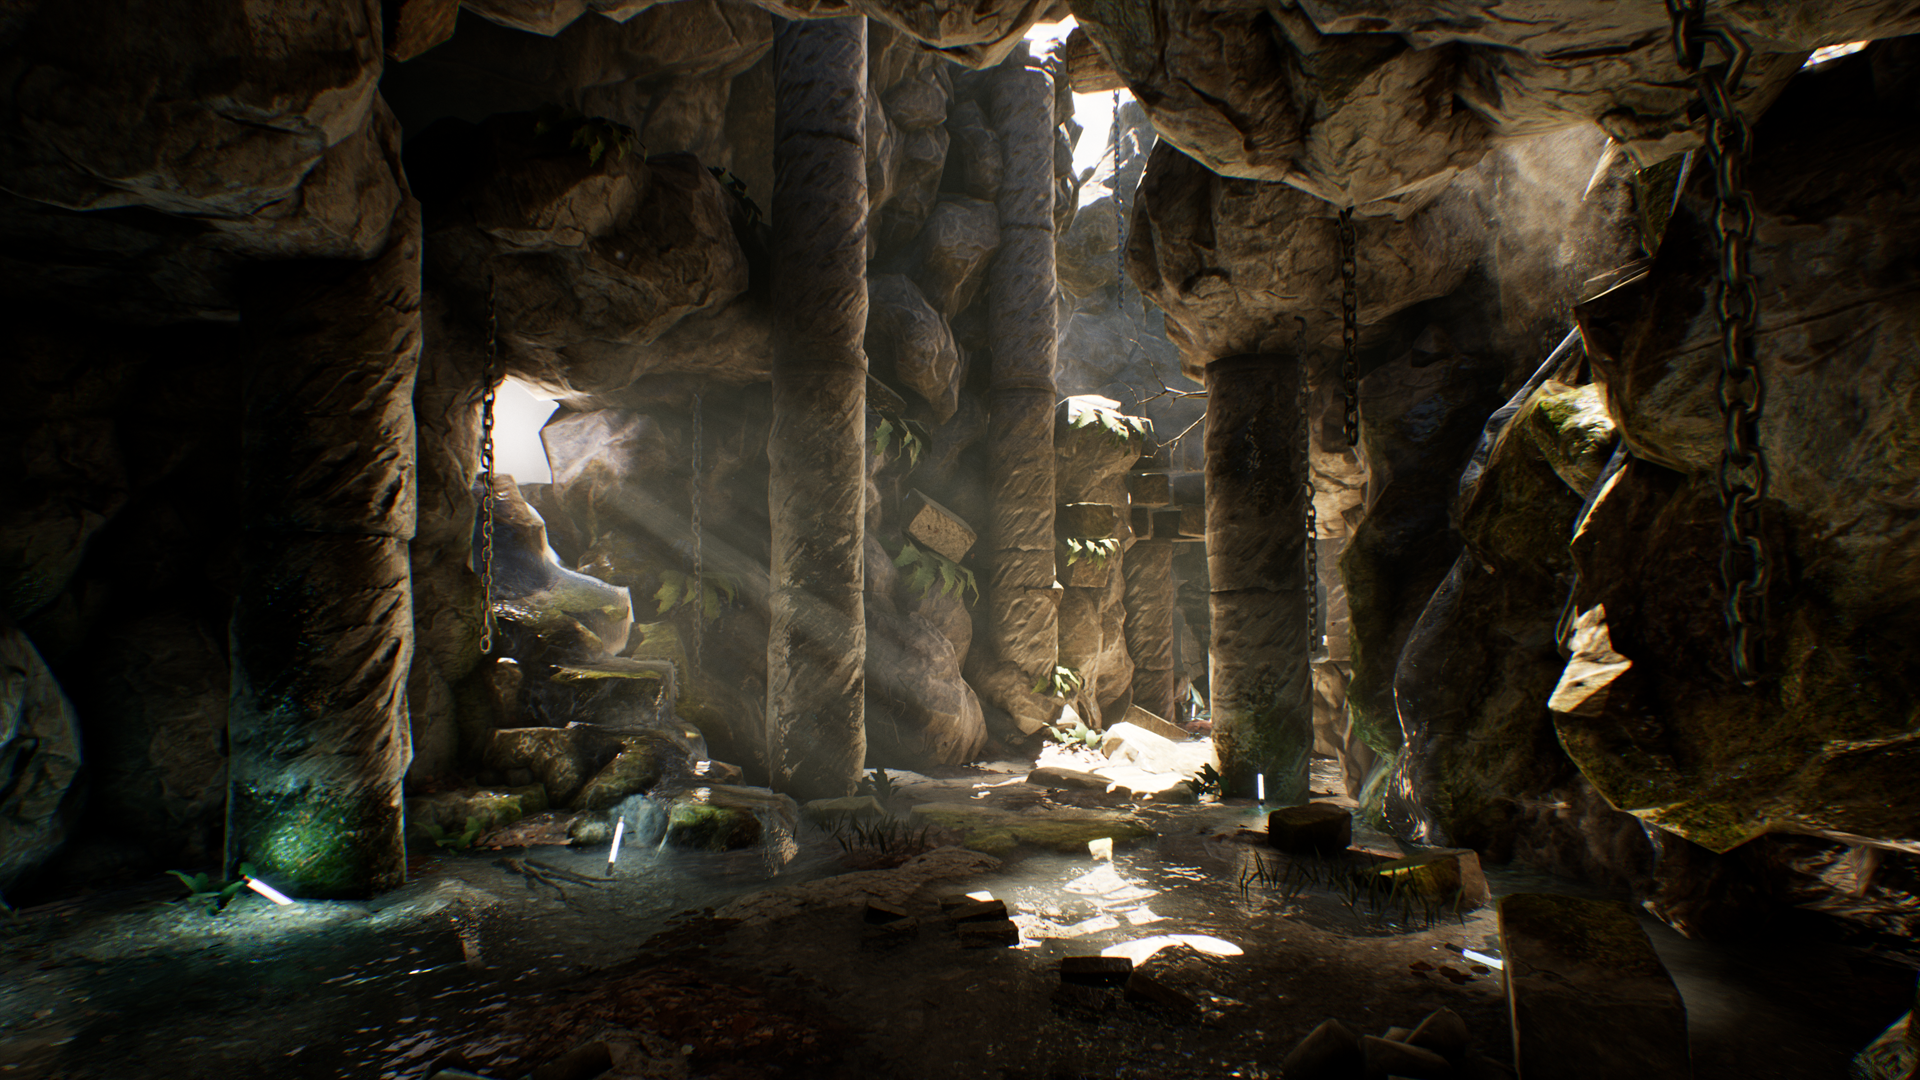
\includegraphics[scale=0.1]{environments/cave.png}

The following environments are only available in Windows
(therefore no significant experiments were done, but usage is possible).

\begin{enumerate}
    \item City.
    \item Africa.
    \item Jing-Zha.
    \item Neighborhood.
\end{enumerate}

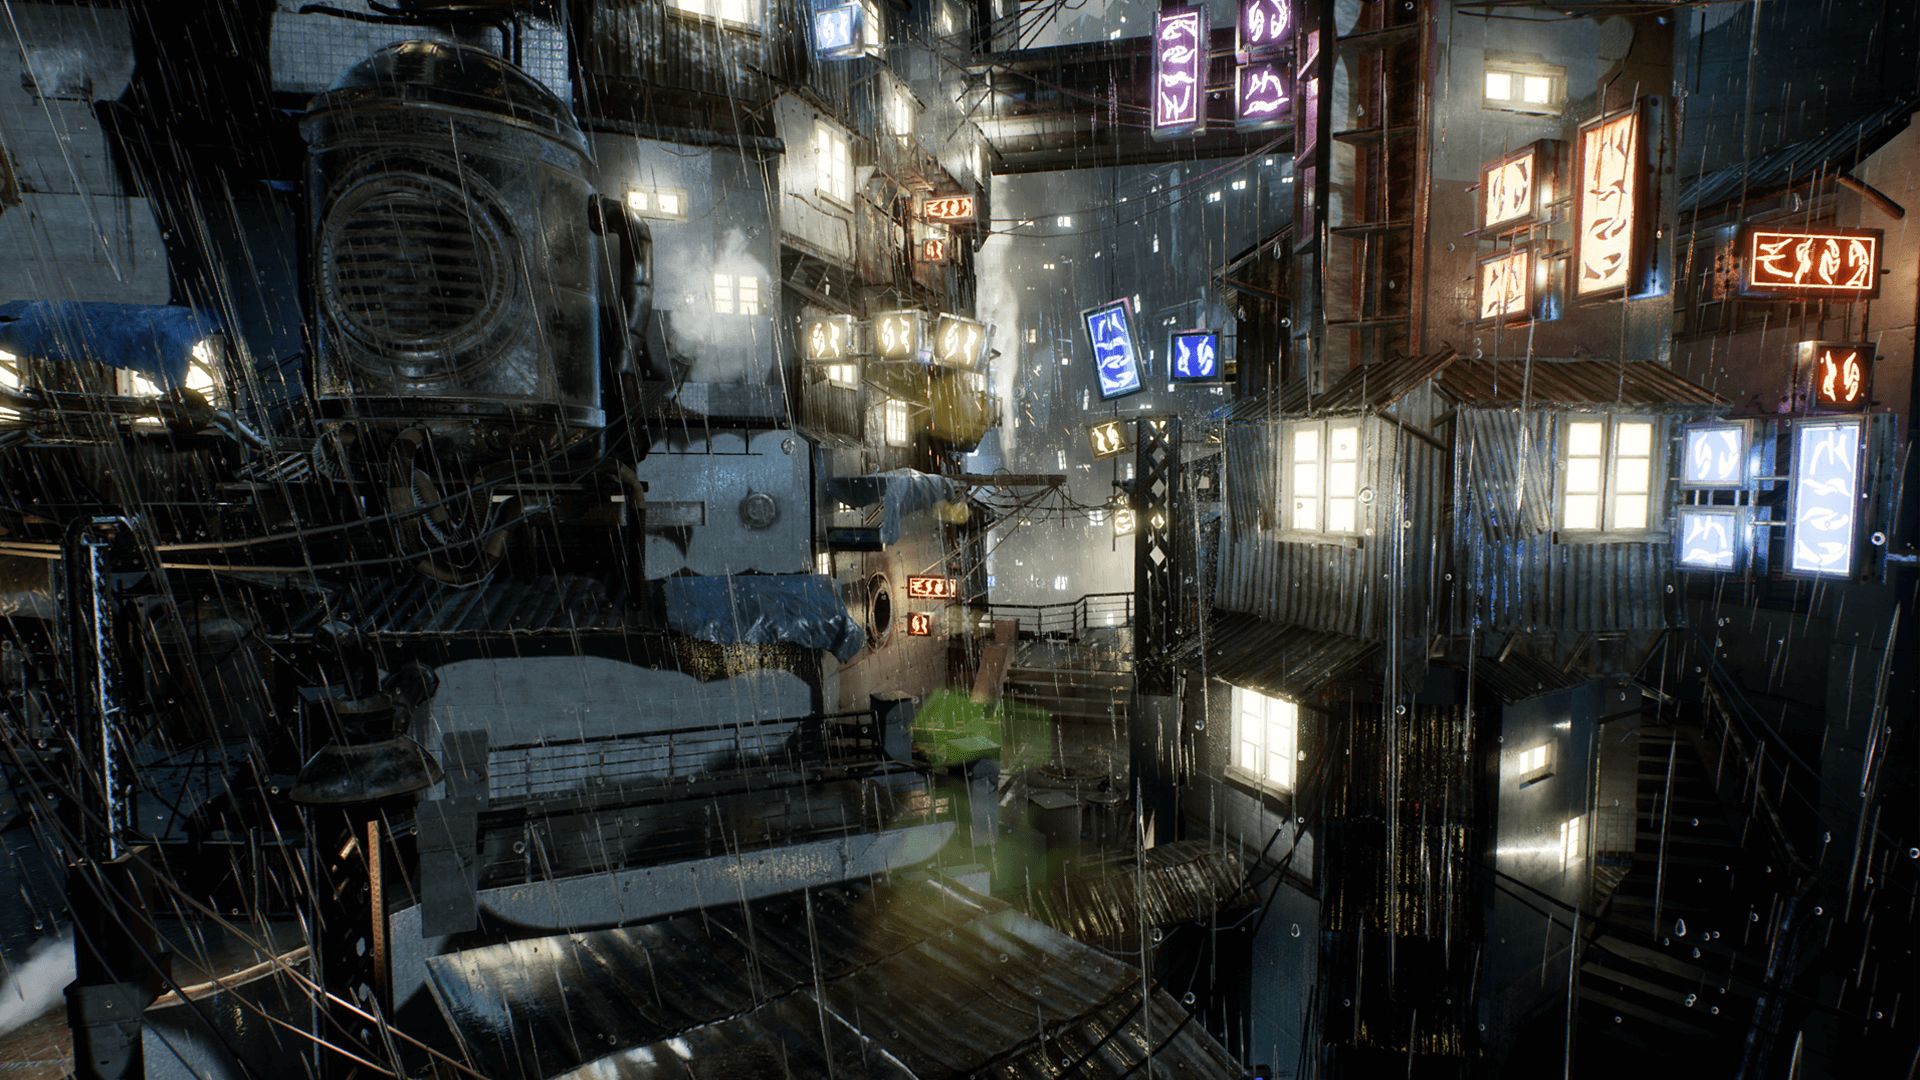
\includegraphics[scale=0.1]{environments/city.png}
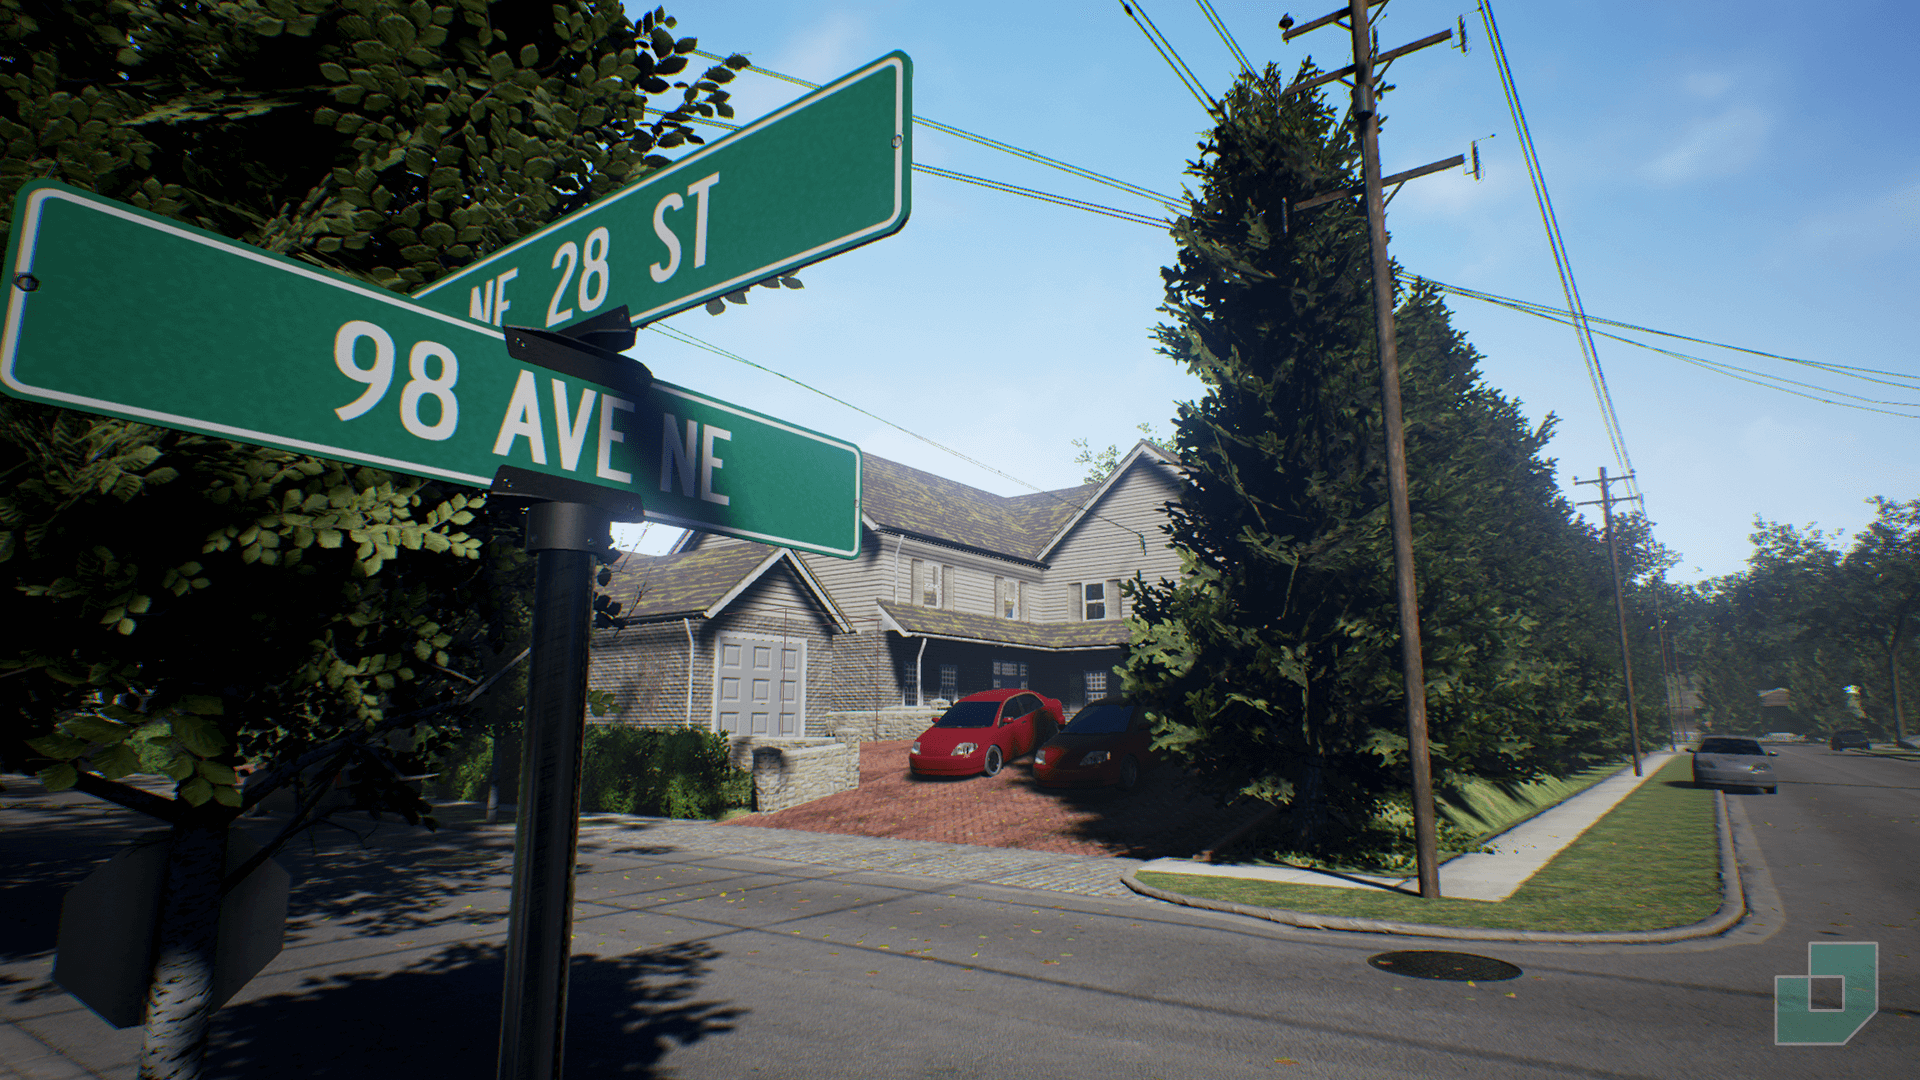
\includegraphics[scale=0.1]{environments/neighborhood.png}


\section{Agent: Deep Q-learning}

\subsection{General description}

We are based on the deep reinforcement
Q-learning, which was first described in \cite{mnih2013playing}.
After a while, more sophisticated version was published in
\cite{mnih2015humanlevel}.

To train the network, standard Q-learning update is converted into the
following loss:

$$L(\theta_i) = \mathbb{E}_{s,a,r,s'} \left[ \left(r + \gamma \max_{a'}Q(s', a'; \theta^{-}) - Q(s, a; \theta_i) \right)^2 \right] $$

\subsection{Network architecture}

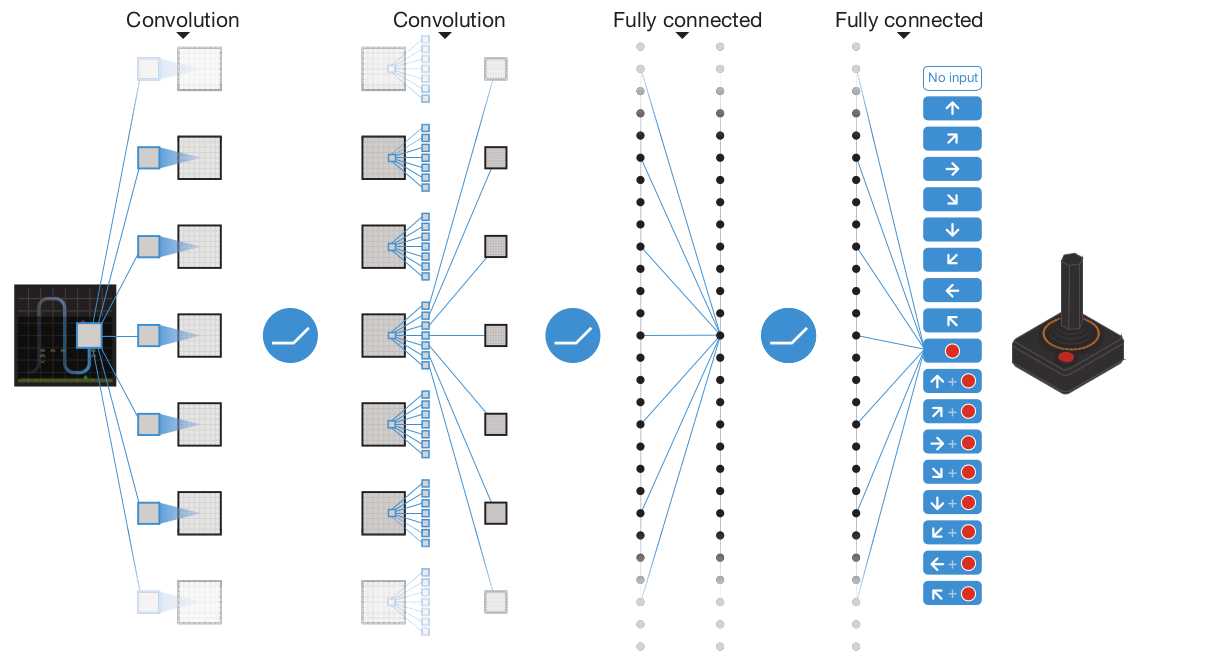
\includegraphics[scale=0.3]{dqn_crop.png}

\subsection{Applied tweaks}

\begin{itemize}
    \item {\bf Experience Replay.} History was collected, and experience was randomly sampled. That helped to reduce correlation in learning.
    \item {\bf Freezed network to reduce correlation.} When computing updates, freezed version was used for estimation. This helps
        to reduce bang of weights.
    \item {\bf Huber Loss.} Huber loss is more robust
        to outliars than MSE.
    \item {\bf 4-frame delayed learning.}
        Taking into account several frames helps network to understand
        distance, velocity and acceleration better.
\end{itemize}

\section{Implemented Rewards}

\begin{itemize}
    \item {\bf Exploration Reward.} Reward is described as $\frac{d - r}{\tau - r}$, where $d$ is distance, $r$ is radius, $\tau$ is constant.
        Also we penalize going too high.
    \item {\bf Path Reward.} We force collision avoidance to fixed lines, and penalize going far wary from them.
    \item {\bf Landscape Reward.} The aim is to reach the goal point in the environment. Therefore the reward is the difference $\text{dist}_{\text{prev}} - \text{dist}$ where $\text{dist}_{\text{prev}}$ is the distance to the goal in the previous state and $\text{dist}$ is distance to the goal in the current state. 
    \item {\bf Corridor Reward.} The reward was inspired by the original paper, as well as  The reward was inspired by the original paper\cite{cad2rl}, as well as some additional considerations about the geometry of a closed space such as a corridor. We try to hardly penalize big changes in altitude(Z axis) as well as reward additional discovery via cityblock distance.  
\end{itemize}

\section{Implemented Action Spaces}

\begin{itemize}
    \item {\bf Grid Action Space.} Frontal camera image is separated into $M^2$ parts, which correspond to moving actions. Moving forward is mandatory.
    \item {\bf Canonical (Default) Action Space.} Forward, Backward, Up, Down, Left, Right, Stay.
    \item {\bf Flat Action Space.} No up or down, rotations introduced.
    \item {\bf Corridor Action Space.} This action space is just a default with added turns to give quadrotor ability to maneuver through the rather tight corners of the corridor. 
\end{itemize}

\section{Exploration}

\begin{itemize}
    \item {\bf Constant $\varepsilon$-greedy.} Exploration is constant over time, or disabled (for evaluation).
    \item {\bf Simulated annealing $\varepsilon$-greedy.} Exploration is scheduled by simulated annealing, and essentially decreases with time.
        Schedule is exponential.
\end{itemize}

Note, that in contrast with using choosing random actions in settings when it almost sertainly leads to some exploration, in our case using uniform probabilities on all actions could result in agent hardly moving, since expectation of such random walk is zero along any chosen axis. Implementing strategy that samples forward movement when exploring with bigger probability resulted in faster learning.  

\section{Results}

Due to file page count limitation, we here present 
only two graphs amoung all working launches (landscape, blocks, corridor, cave).
All other graphs can be found in our github repository, and look similar.

Corridor:
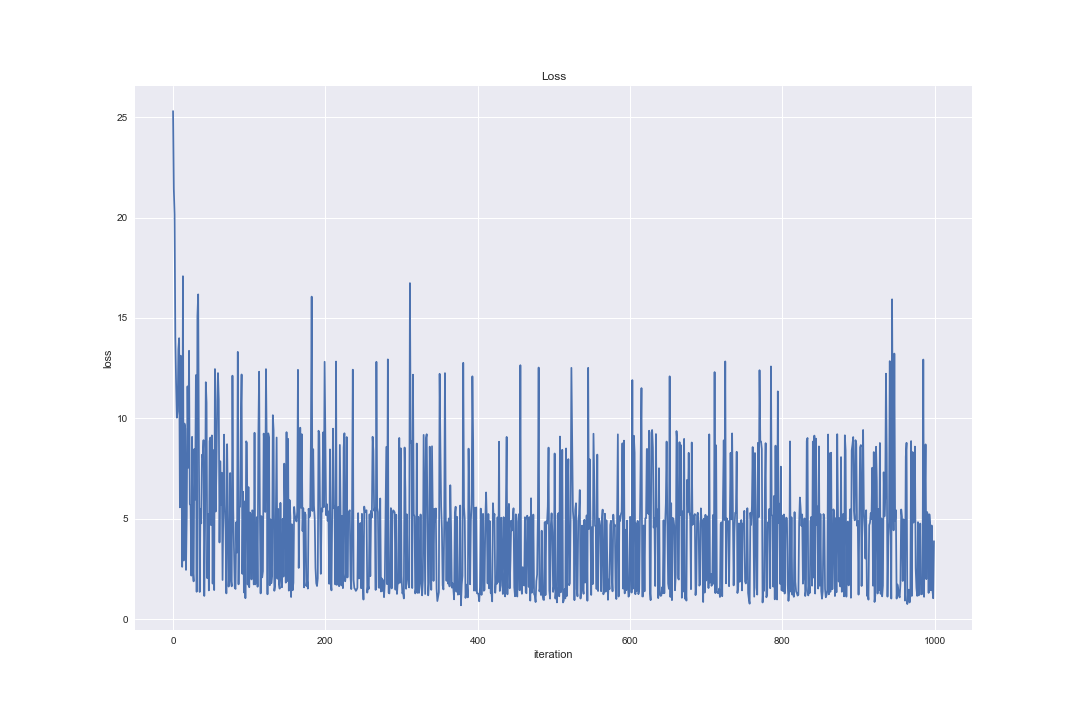
\includegraphics[scale=0.2]{plots/corridor_loss.png}
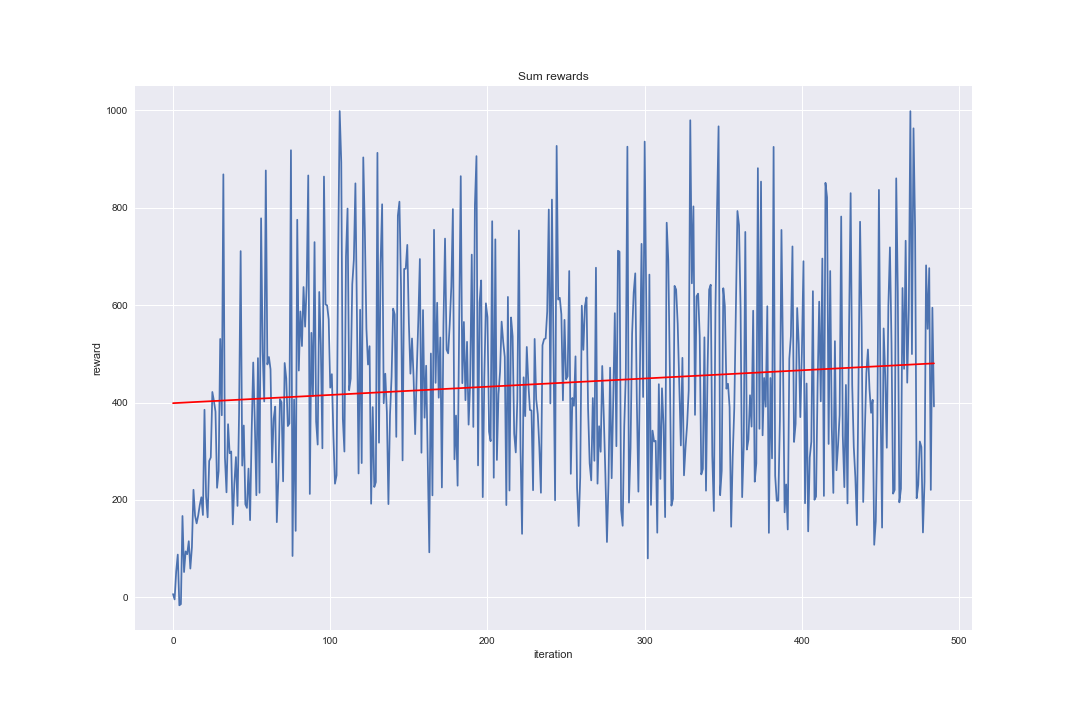
\includegraphics[scale=0.2]{plots/corridor_rewards.png}

Landscape:

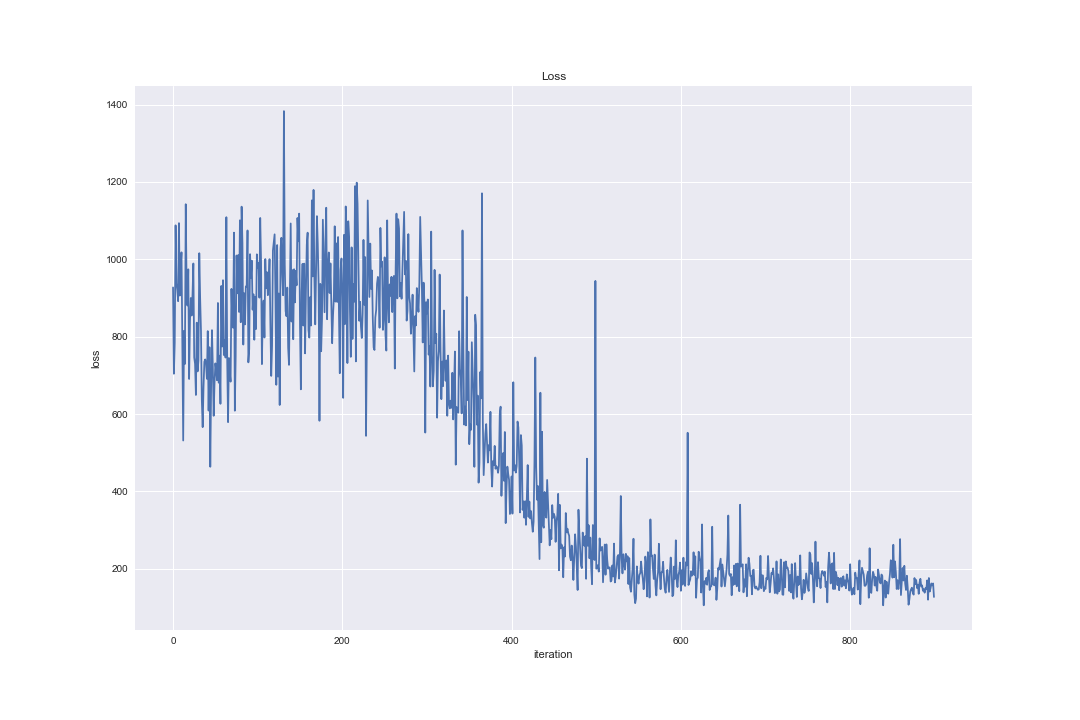
\includegraphics[scale=0.2]{plots/landscape_loss.png}
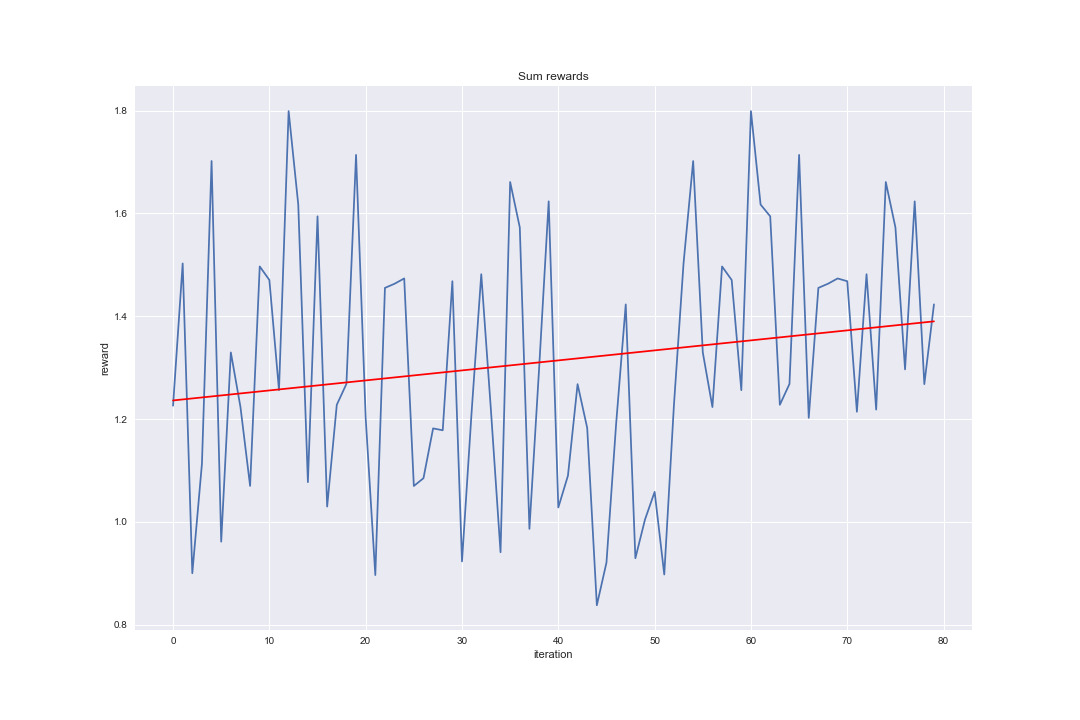
\includegraphics[scale=0.2]{plots/landscape_rewards.png}

\bibliographystyle{unsrt}
\bibliography{reference}

\end{document}
